%
% File acl2019.tex
%
%% Based on the style files for ACL 2018, NAACL 2018/19, which were
%% Based on the style files for ACL-2015, with some improvements
%%  taken from the NAACL-2016 style
%% Based on the style files for ACL-2014, which were, in turn,
%% based on ACL-2013, ACL-2012, ACL-2011, ACL-2010, ACL-IJCNLP-2009,
%% EACL-2009, IJCNLP-2008...
%% Based on the style files for EACL 2006 by 
%%e.agirre@ehu.es or Sergi.Balari@uab.es
%% and that of ACL 08 by Joakim Nivre and Noah Smith

\documentclass[11pt,a4paper]{article}
\usepackage[hyperref]{acl2019}
\usepackage{times}
\usepackage{latexsym}
\usepackage{url}
\usepackage{graphicx}

\aclfinalcopy % Uncomment this line for the final submission
%\def\aclpaperid{***} %  Enter the acl Paper ID here

%\setlength\titlebox{5cm}
% You can expand the titlebox if you need extra space
% to show all the authors. Please do not make the titlebox
% smaller than 5cm (the original size); we will check this
% in the camera-ready version and ask you to change it back.

\newcommand\BibTeX{B\textsc{ib}\TeX}

\title{Survey of techniques for domain specific Named Entity Recognition}

\author{Manik Bhandari \\
  Indian Institute of Science \\
  % Affiliation / Address line 2 \\
  % Affiliation / Address line 3 \\
  \texttt{manikb@iisc.ac.in} \\
  }
  % \And
  % Second Author \\
  % Affiliation / Address line 1 \\
  % Affiliation / Address line 2 \\
  % Affiliation / Address line 3 \\
  % \texttt{email@domain} \\}

\date{}

\begin{document}
\maketitle
\newcommand{\refalg}[1]{Algorithm \ref{#1}}
\newcommand{\refeqn}[1]{Equation \ref{#1}}
\newcommand{\reffig}[1]{Figure \ref{#1}}
\newcommand{\reftbl}[1]{Table \ref{#1}}
\newcommand{\refsec}[1]{Section \ref{#1}}
%\newcommand{\method}[1]{\mbox{\textsc{#1}}}

\newcommand{\reminder}[1]{\textcolor{red}{[[ #1 ]]}\typeout{#1}}
\newcommand{\reminderR}[1]{\textcolor{gray}{[[ #1 ]]}\typeout{#1}}

\newcommand{\add}[1]{\textcolor{red}{#1}\typeout{#1}}
\newcommand{\remove}[1]{\sout{#1}\typeout{#1}}

\newcommand{\m}[1]{\mathcal{#1}}
\newcommand{\method}{Syntactic-BERT}

\newtheorem{theorem}{Theorem}[section]
\newtheorem{claim}[theorem]{Claim}

\newcommand{\tensor}{\mathcal{X}}
\newcommand{\Real}{\mathbb{R}}

\newcommand{\tuples}{\mathbb{T}}

% \newcommand{\argmax}{arg\,max}

\newcommand\norm[1]{\left\lVert#1\right\rVert}

\newcommand{\note}[1]{\textcolor{blue}{#1}}

\newcommand*{\Scale}[2][4]{\scalebox{#1}{$#2$}}%
\newcommand*{\Resize}[2]{\resizebox{#1}{!}{$#2$}}%

%%% Tensor
%\DeclareMathAlphabet\ten{OMS}{cmsy}{b}{n} %%usage: \mathbfcal{W}
%% Matrix
\def\mat#1{\mbox{\bf #1}}%% usage: \mat{W}.

\begin{abstract}
    This document is a brief summary of relevant work in the field of domain-
    specific Named Entity Recognition (NER).
\end{abstract}


\section{Introduction}
\label{sec:intro}
\subsection{Define the problem}

\subsection{Major Challenges}
\begin{enumerate}
	\item Lack of corpus.
	\item Lack of supervised NER tags - you have to manually define the set of entities that you are interested in so this set will always be small. 
	\item Disambiguation - same surface form can mean two things in different context.
\end{enumerate}

\section{Summary of Papers}
\label{sec:summary}

\subsection{AutoNER}
AutoNER \cite{autoner} is the recent SOTA in domain-specific NER. It has two contributions: Fuzzy LSTM CRF and Tie-or-Break scheme.
\\

\noindent\textbf{Tie-or-Break Scheme}
In a sentence, predict whether two words should be tied together to form one phrase or broken apart. Now, between every to 'breaks' you have a potential named entity. Predict its type ('None' being the type that it's not a named entity).

Training data for these phrases comes from another paper of the same group \cite{autophrase} which uses unsupervised methods to extract interesting phrases from a large corpus.
\\

\noindent\textbf{Fuzzy LSTM CRF}
Have to read about CRF and how they work. 
\begin{enumerate}
	\item Neither BERT nor ELMO use CRF and both report SOTA results on NER.
	\item Need to check if CRFs work for domain specific case? If so, why?
\end{enumerate}

They also introduce a training mechanism which models the noise in supervision.
Let $v_i$ be the vector for a phrase (constructed using concatenation of beginning and ending word). Pass it through a softmax layer to get 

\[
	p(t_j|v_i) = \frac{e^{t_j^Tv_i}}{\sum_{k}{e^{t_k^Tv_i}}}
\]

Usually, you would now take a cross-entropy loss. But since a word can belong to multiple types, define
\[
	\hat{p}(t_j|v_i) = \frac{\delta(s_i \in t_j) e^{t_j^Tv_i}}{\sum_{k}{\delta(s_i \in t_k)e^{t_k^Tv_i}}}
\]

where $\delta$ is a boolean function which checks whether the span $s_i$ is ever marked with type $t_j$ in distant supervision.

Now take cross-entropy loss between $p$ and $\hat{p}$.

The only difference between $\hat{p}$ and $p$ is that to get $\hat{p}$ you mask the values of $p$ that are never assigned in distant supervision. 

Essentially this punishes the model if it gives any weight to those values and allows the model to learn whatever it wants for the probable types.

\reminder{Maybe there's something wrong here.} But if the above is true, the model never gets to see the true type in the current context. How will the model learn to disambiguate?


\begin{figure*}[t]
	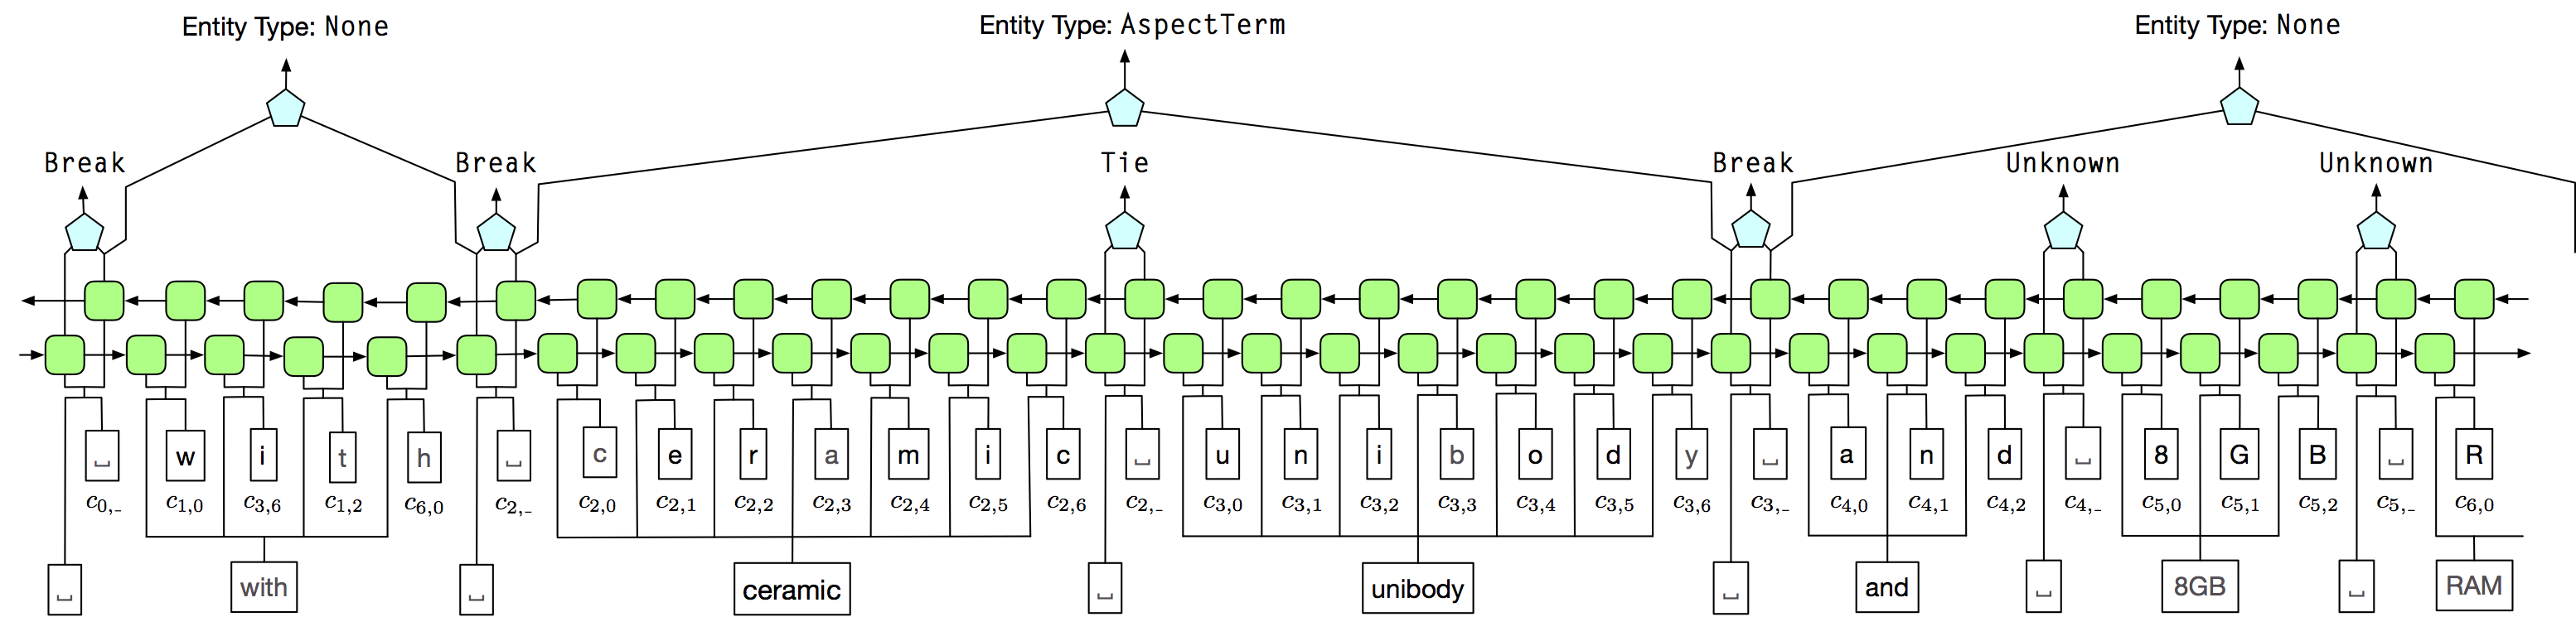
\includegraphics[scale=0.3]{images/autoner_tie_or_break.png}
	\caption{\label{fig:tie_or_break}Overview of the Tie-or-Break scheme used in AutoNER.}
\end{figure*}

\subsection{Character Level Language Modeling}
\begin{enumerate}
	\item Character level features are important for NER. For instance, first letter being capitalized implies a proper noun, names of places in North India typically end in '-pur' (like Jaipur, Raipur) etc.
	\item For char-level LM, sequence lengths become too large to be directly fed into a Transformer Network. Naive solution is to break a sequence down into shorter pieces but then you lose context. One way to retain context is to keep a \textit{memory} and use that to remember earlier parts of a sequence \cite{transformerxl}.
	\item I struggled with the code of this paper. Decided to first test the hypothesis on standard BERT and if there is potential, use it for such a character-level language model as well.
\end{enumerate}

\begin{figure*}[t]
	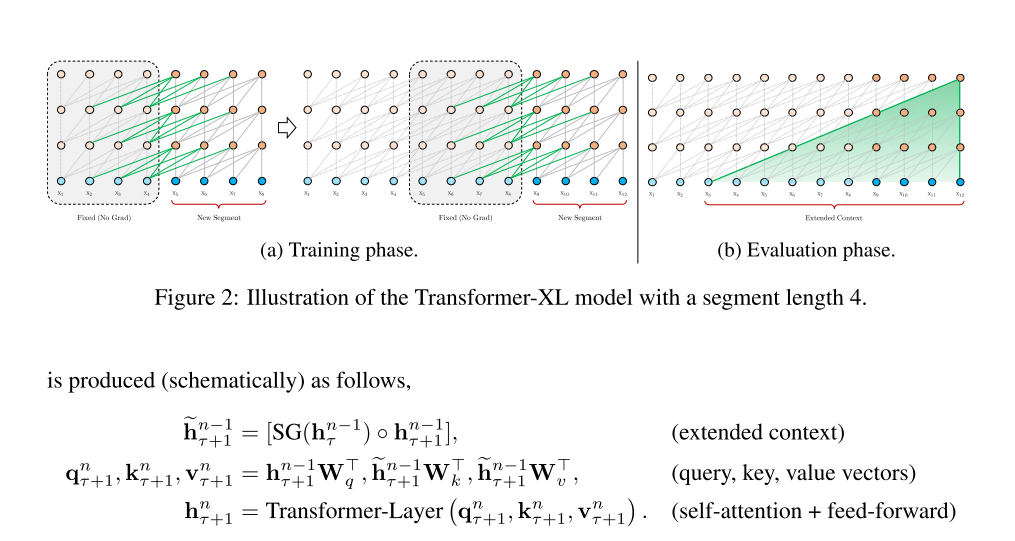
\includegraphics[scale=0.5]{images/transformerxl}
	\caption{\label{fig:transformerxl}Overview of transformer-xl which uses extended context to solve the problem of sending large sequences through Transformers.}
\end{figure*}


\section{Proposed Method}
\label{sec:proposed_method}
\method{} solves all three major challenges.
\begin{enumerate}
	\item Using transfer learning, we avoid the problem of lack of a huge corpus for getting contextualized embeddings.
	\item We use additional low-level, syntactic tasks which provide low level supervision and force the model to learn syntactic information. This syntactic information like POS tags can be used by the model to predict Named Entities \cite{autoner} \reminder{Also cite POS paper}.
	\item We use distant supervision paradigm and use \textit{soft supervision} as described in AutoNER to allow our model to learn \textit{soft labels}.
\end{enumerate}
\section{Experiments}
\label{sec:experiments}
\section{Discussion}
\label{sec:discussion}

\begin{enumerate}
	\item Preliminary experiments suggest that training BERT from scratch on a small corpus (~20K sentences) is bad. This is a little surprising (but kind of expected) because the vocabulary size of this corpus is only around 10K.
	\item Next in performance is Pretrained BERT without any language modeling fine tuning. Best so far (apart form SOTA) is BERT with language model fine tuning to domain specific corpus.
\end{enumerate}

\bibliographystyle{acl_natbib}
\bibliography{acl2019.bib}
\end{document}
